\chapter{Βιβλιογραφία}

%Το \en{Lorem Ipsum} είναι απλά ένα κείμενο χωρίς νόημα για τους επαγγελματίες της τυπογραφίας και στοιχειοθεσίας \cite{LoremIpsumAll}. Το \en{Lorem Ipsum} είναι το επαγγελματικό πρότυπο όσον αφορά το κείμενο χωρίς νόημα, από τον 15ο αιώνα, όταν ένας ανώνυμος τυπογράφος πήρε ένα δοκίμιο και ανακάτεψε τις λέξεις για να δημιουργήσει ένα δείγμα βιβλίου. Όχι μόνο επιβίωσε πέντε αιώνες, αλλά κυριάρχησε στην ηλεκτρονική στοιχειοθεσία, παραμένοντας με κάθε τρόπο αναλλοίωτο. Έγινε δημοφιλές τη δεκαετία του '60 με την έκδοση των δειγμάτων της \en{Letraset} όπου περιελάμβαναν αποσπάσματα του \en{Lorem Ipsum}, και πιο πρόσφατα με το λογισμικό ηλεκτρονικής σελιδοποίησης όπως το \en{Aldus PageMaker} που περιείχαν εκδοχές του \en{Lorem Ipsum}.


\section{Βιβλιογραφίκές αναφορές}
\begin{itemize}
    \item [1] \en{https://kubernetes.io/docs/concepts/overview/}  
    \item [2] \en{Vs Code development environment}
    \item [3] \en{https://el.wikipedia.org/wiki/}
    \item [4] \en{Virtual box} \en{https://www.virtualbox.org/manual/}
    \item [5] \en{https://www.cloudflare.com/learning/network-layer/what-is-the-control-plane/}
    \item [6] \en{https://el.wikipedia.org/wiki/Git}
    \item [7] \en{https://kubernetes.io}
    \item [8] \en{https://github.com/dmfigol/network-programmability-stream}
    \item [9] \en{https://medium.com/@komalminhas.96/a-step-by-step-guide-to-build-and-push-your-own-docker-images-to-dockerhub-709963d4a8bc}
    \item [10] \en{https://repository.ihu.edu.gr/}, \en{Network automation using python George Milios}
    \item [11] \en{Wikipedia}, τι είναι το \en{Windows Subsystem for Linux}
    \item [12] \en{wikipedia.org/wiki/Modelviewcontroller}
    \item [13] \en{https://docs.docker.com/engine/daemon/start/}
    \item [14] \en{https://minikube.sigs.k8s.io/docs/start/}
    \item [15] \en{https://developer.mozilla.org/en-US/docs/Glossary/MVC}
    \item [16] \en{https://www.freecodecamp.org/news/python-requirementstxt-explained/}
    \item [17] \en{https://kubernetes.io/docs/tutorials/hello-minikube/}
    \item [18] \en{https://kubernetes.io/docs/tasks/run-application/horizontal-pod-autoscale/}
    \item [19] \en{https://docs.gns3.com/docs/using-gns3/advanced/connect-gns3-internet/}
    \item [20] \en{https://github.com/hegdepavankumar/Cisco-Images-for-GNS3-and-EVE-NG}
    \item [21] \en{https://www.paramiko.org/}
    \item [22] \en{https://github.com/ktbyers/netmiko}
    \item [23] \en{https://napalm.readthedocs.io/en/latest/index.html}
    \item [24] \en{https://www.ericsson.com/en/portfolio/cloud-software-and-services/network-management-and-automation/ericsson-network-manager}
    \item [25] \en{https://www.sitepoint.com/wsl2/}
    \item [26] \en{https://docs.gns3.com/docs/using-gns3/beginners/import-gns3-appliance/}
\end{itemize}


%\begin{equation}
%	y = \alpha x + \beta
%\end{equation}

%Αντίθετα με αυτό που θεωρεί η πλειοψηφία, το \en{Lorem Ipsum} δεν είναι απλά ένα τυχαίο κείμενο. Οι ρίζες του βρίσκονται σε ένα κείμενο Λατινικής λογοτεχνίας του 45 π.Χ., φτάνοντας την ηλικία του πάνω από 2000 έτη.


%\begin{figure}[htb]
%	\centering
%	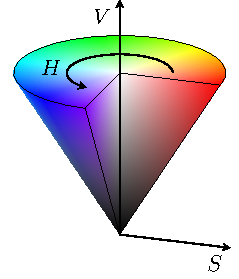
\includegraphics{tikz/hsv_cone/hsv_cone.pdf}
%	\caption{Ο χρωματικός χώρος \en{HSV}.}
%\end{figure}
